% =====================================================================
% HÌNH TikZ — thay Fig.1 và Fig.2. 2026-09-30.
% Số thật: full 97.99 / mean-pool 95.77 / no-hier 89.62.
% =====================================================================

% ---------------------------------------------------------------------
% PREAMBLE: thêm vào đầu bài (sau các \usepackage khác), nếu chưa có:
% ---------------------------------------------------------------------
% \usepackage{tikz}
% \usepackage{pgfplots}
% \pgfplotsset{compat=1.16}
% \usetikzlibrary{arrows.meta, positioning, fit, backgrounds, calc}

% ---------------------------------------------------------------------
% FIG.1 — Pipeline kiến trúc H-GNN (thay \begin{figure*}...Fig1.pdf...\end{figure*})
% Nhiệm vụ nhị phân (Benign/Malicious), KHÔNG có "family", KHÔNG có số accuracy.
% ---------------------------------------------------------------------
\begin{figure*}[t]
\centering
\begin{tikzpicture}[
  font=\small,
  >={Stealth[length=2mm]},
  stage/.style={draw, rounded corners=2pt, align=center, minimum height=1.05cm,
                text width=2.75cm, fill=blue!5, thick},
  io/.style={draw, align=center, minimum height=1.0cm, text width=1.9cm, fill=gray!8},
  lvl/.style={draw, dashed, rounded corners=3pt, inner sep=6pt},
  arr/.style={->, thick},
]
% input
\node[io] (bin) {Multi-arch\\ ELF binaries\\ \scriptsize(ARM/MIPS/PPC/x86)};
% stage 1
\node[stage, right=0.9cm of bin] (lift) {\textbf{Stage 1}\\ Architecture-agnostic\\ VEX~IR lifting (angr)};
% stage 2
\node[stage, right=0.9cm of lift] (graph) {\textbf{Stage 2}\\ Hierarchical graph\\ construction\\ \scriptsize(bounded CFG + ICG)};
% stage 3
\node[stage, right=0.9cm of graph] (gnn) {\textbf{Stage 3}\\ Hierarchical neural\\ aggregation};
% output
\node[io, right=0.9cm of gnn, fill=green!8] (out) {Decision:\\ \textbf{Benign} /\\ \textbf{Malicious}};

\draw[arr] (bin) -- (lift);
\draw[arr] (lift) -- (graph);
\draw[arr] (graph) -- (gnn);
\draw[arr] (gnn) -- (out);

% chi tiết 2 cấp dưới Stage 2/3
\node[draw, rounded corners=2pt, below=1.0cm of graph, text width=3.0cm, align=center, fill=orange!8, font=\scriptsize]
  (l1) {\textbf{Level 1: Intra-CFG}\\ per-function VEX-statement\\ graphs, $K_{\max}{=}50$ funcs,\\ $\le 200$ stmts/func};
\node[draw, rounded corners=2pt, below=1.0cm of gnn, text width=3.0cm, align=center, fill=orange!8, font=\scriptsize]
  (l2) {\textbf{Level 2: Inter-ICG}\\ call graph from VEX\\ transfer primitives\\ (no symbol table)};
\draw[arr, gray] (graph) -- (l1);
\draw[arr, gray] (gnn) -- (l2);

\node[draw, rounded corners=2pt, below=0.35cm of l1, text width=3.0cm, align=center, fill=purple!6, font=\scriptsize]
  (p1) {GATv2 + local max-pool\\ $\rightarrow$ function embeddings};
\node[draw, rounded corners=2pt, below=0.35cm of l2, text width=3.0cm, align=center, fill=purple!6, font=\scriptsize]
  (p2) {GraphSAGE + global\\ max-pool $\rightarrow$ program vector};
\draw[arr, gray] (l1) -- (p1);
\draw[arr, gray] (l2) -- (p2);
\end{tikzpicture}
\caption{Overview of the proposed \text{H-GNN} framework. Heterogeneous
multi-architecture ELF binaries are lifted into architecture-agnostic VEX
IR, decomposed into a two-level hierarchical graph (bounded
intra-procedural CFGs and an inter-procedural call graph reconstructed
from control-flow primitives), and encoded bottom-up with GATv2 and
GraphSAGE for binary malware detection at the edge.}
\label{fig:system_overview}
\end{figure*}

% ---------------------------------------------------------------------
% FIG.2 — Ablation bar chart (thay \begin{figure}...Fig2.pdf...\end{figure})
% Số thật từ 5-seed (full, mean-pool) và 2-seed (no-hier).
% ---------------------------------------------------------------------
\begin{figure}[!t]
\centering
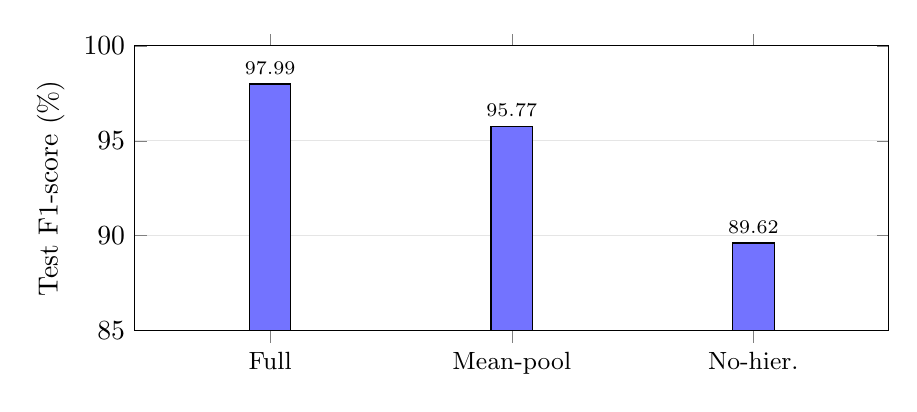
\begin{tikzpicture}
\begin{axis}[
  ybar,
  width=0.92\columnwidth,
  height=5.2cm,
  bar width=15pt,
  ymin=85, ymax=100,
  ylabel={Test F1-score (\%)},
  symbolic x coords={Full, {Mean-pool}, {No-hier.}},
  xtick=data,
  x tick label style={font=\small, align=center},
  nodes near coords,
  nodes near coords style={font=\scriptsize},
  every node near coord/.append style={/pgf/number format/precision=2, /pgf/number format/fixed},
  enlarge x limits=0.28,
  ymajorgrids=true, grid style=gray!20,
]
\addplot[fill=blue!55] coordinates {(Full,97.99) ({Mean-pool},95.77) ({No-hier.},89.62)};
\end{axis}
\end{tikzpicture}
\caption{Component ablation (test F1-score). The full \text{H-GNN} with
hierarchical decomposition and global max-pooling attains
\hgnnF\%; replacing global max-pooling with mean-pooling drops it to
\ablMean\%, and removing the hierarchical decomposition drops it to
\ablNoHier\% (mean of two seeds), confirming both design choices.}
\label{fig:ablation_study}
\end{figure}

% ---------------------------------------------------------------------
% CÁCH ÁP:
% 1. Thêm 4 dòng preamble (tikz, pgfplots, compat, usetikzlibrary) nếu chưa có.
% 2. Xóa khối \begin{figure*}...includegraphics{Figs/Fig1.pdf}...\end{figure*}
%    thay bằng khối FIG.1 ở trên.
% 3. Xóa khối \begin{figure}...includegraphics{Figs/Fig2.pdf}...\end{figure}
%    thay bằng khối FIG.2 ở trên.
% 4. pdflatex 2 lần. Không cần Figs/*.pdf nữa.
% Nếu pgfplots báo lỗi version, đổi compat=1.16 thành số phù hợp (thử 1.18).
% ---------------------------------------------------------------------
